% status: 0
% chapter: TBD

\title{HPCC Systems}

\author{Hao Tian}
\affiliation{%
  \institution{Indiana University}
  \streetaddress{School of Informatics, Computing and Engineering}
  \city{Bloomington} 
  \state{IN} 
  \postcode{47408}
  \country{USA}}
\email{tian4@indiana.edu}


% The default list of authors is too long for headers}
\renewcommand{\shortauthors}{H. Tian.}


\begin{abstract}

HPCC (High Performance computer cluster) systems are open source tool which offers the BigData related services. HPCC contains tools that deal with complex data structure and large scale of data amount. It is a powerful open source tool for data analyze, especially for the significant size of data. The functionalities of HPCC such as fast querying to different databases, , data visualization, and data management have good reputation to many users.

One of the properties of the HPCC system is easy-to-used; it is easy to learn from a developer side, and it also contains exhaustive resources for a beginner to learn. For example, the HPCC has free training and completed documentation for the new user, and even user has some unexperienced issue which is hard to solve, the development community can also help the user to learn. Despite it is easy to use, the powerful computing mechanism of the system and the massive cloud computing platform bring the HPCC system supercomputing capability.

This paper discusses the general functionality of the HPCC system, and the paper further discusses the basic mechanism of the HPCC system, finally conclude the advantages of the system compare with other cloud computing systems. In section 1 and section 2, the papers introduces the basic functionality of the HPCC system. In the section 3, the papers discusses the core mechanism of the HPCC system, and analyzes the components of the system which could bring advantages of different perspectives to the HPCC system. In conclusion, the paper summarizes the functionalities, mechanisms, and advanced properties of the HPCC system.
\end{abstract}

\keywords{hid-sp18-524, High-performance computing, Clusters, Big data, Open Source, Parallel Computing}

\maketitle

\section{Introduction}

The HPCC system is a open source platform which serves Big Data analyzing, the platform that could handles any data scale and very easy to use. it was developed by LexisNexis\textsuperscript{\textregistered} Risk Solutions for large scale data analyzing, and gradually become an open source project from different development team to makes the system better. Because of the powerful supporting from open source development teams and well maintenance from all different supporters, the HPCC system is a powerful tool for data engineers to process raw data, and also for data scientists to analyze data in order to gather useful information. The HPCC system has great reputation in the data analyzing area, it is not only because of the efficiency of the system, but also because the HPCC system is complete free~\cite{Intro1}.

The HPCC system, as what the name represents, the HPCC stands for \textit{High Performance computer cluster}; it is the main component, or the core of the system platform. The HPCC main component includes three platforms that work together to achieve high performance computing: (The Figure ~\ref{f:hpcc} shows the general structure of the HPCC system)

\begin{figure}[!ht]
\centering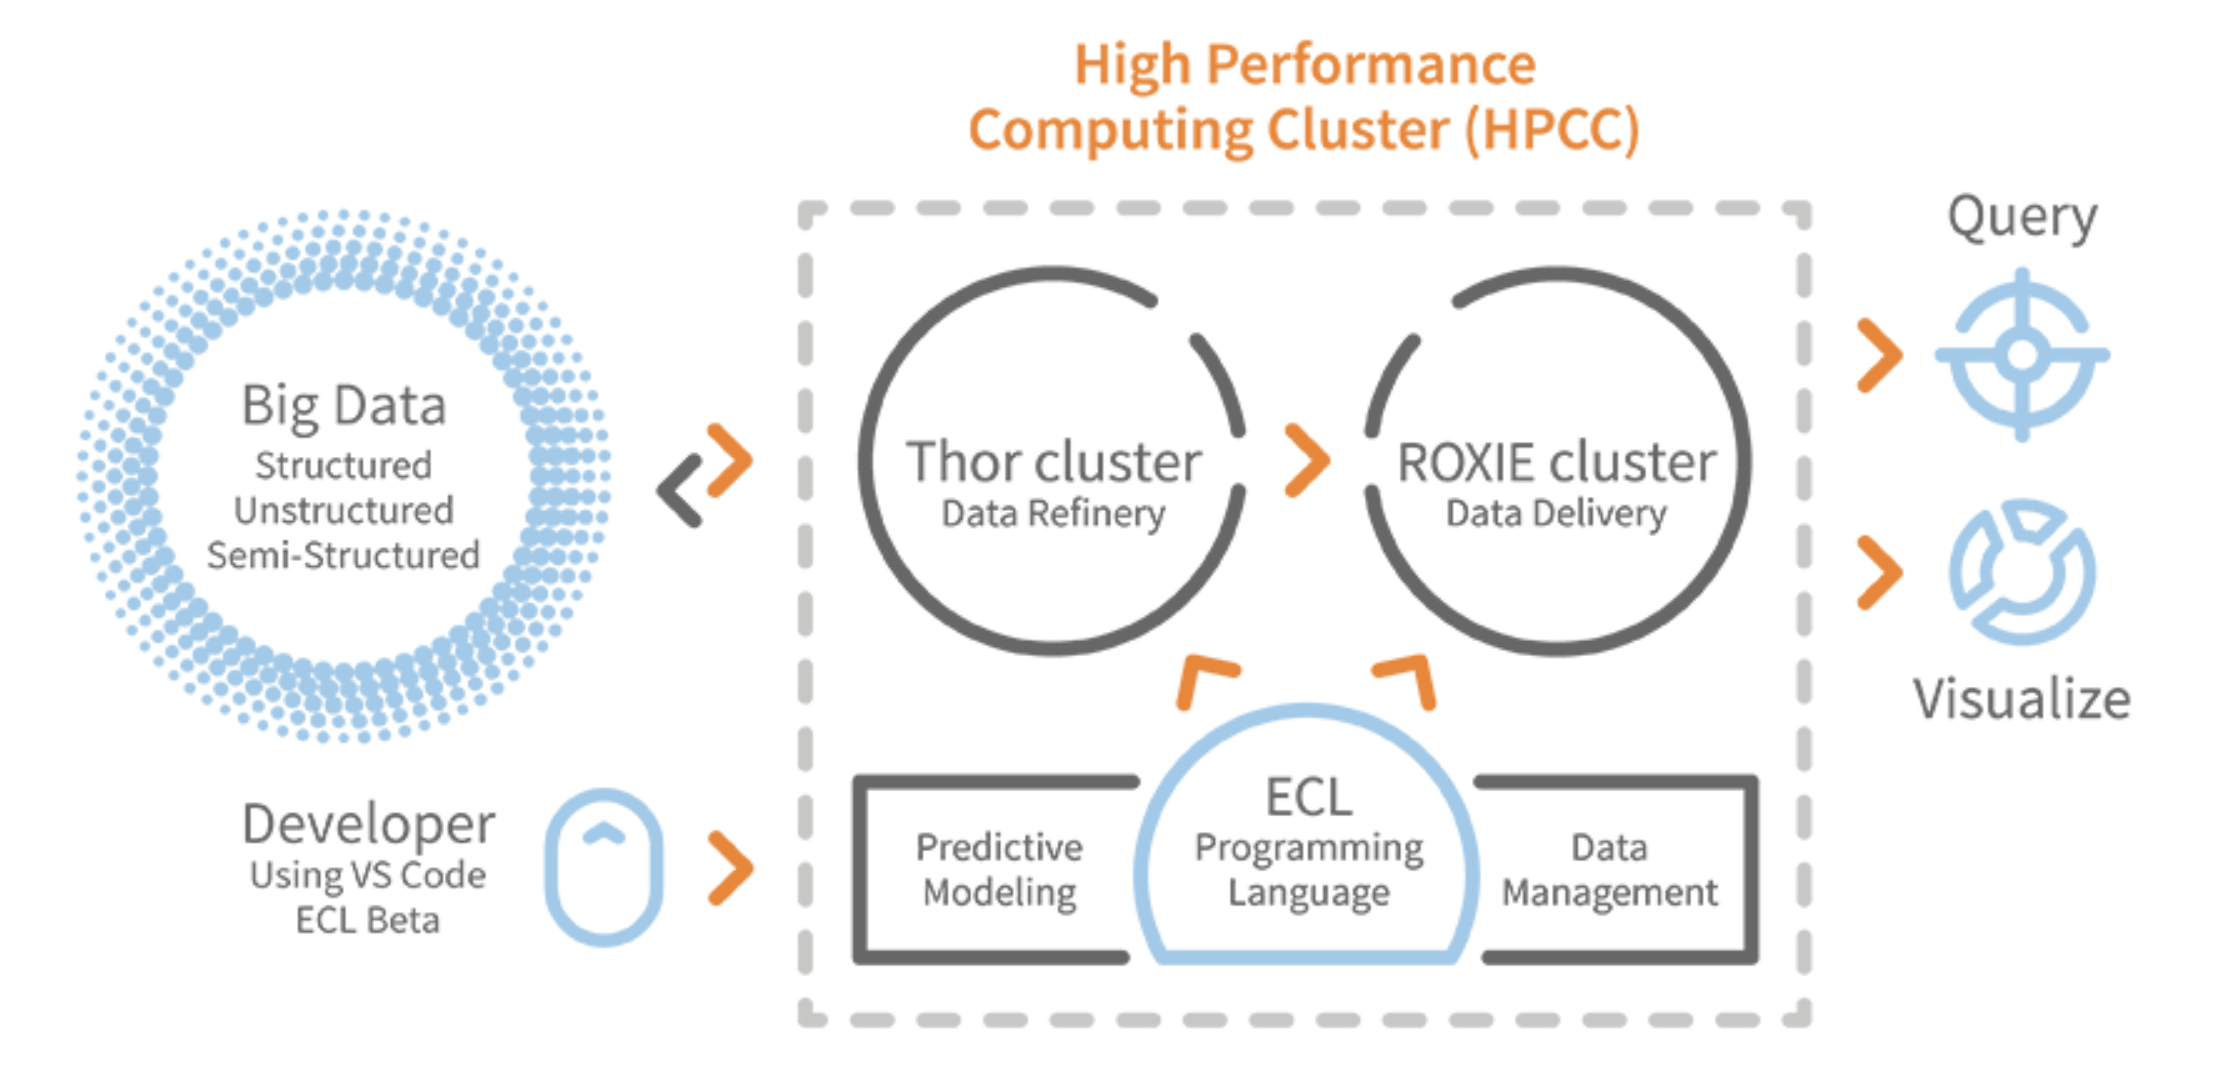
\includegraphics[width=\columnwidth]{images/hpcc.png}
\caption{The basic HPCC structure}\label{f:hpcc}
\end{figure}

\begin{itemize}
	\item Thor system clusters for data refinery: it includes data management, data cleaning and other functionalities for processing raw data ~\cite{Intro3}.
	\item Roxie system clusters for data delivery: it use rapid search engine to get specific data record. it is the main component for the data analyzing and query developing~\cite{HPCC}.
	\item the ECL Programming Language platform: it is a special programming language bases on C++, which gives the developers a visualized form to modify methods for data analyzing with their own purposes. The HPCC is driven by ECL~\cite{Intro2}.
\end{itemize}

The first two components, Thor and Roxie systems, are the main components for achieving high performance computing of the system. for HPCC system that serves companies data analyzing, the Thor collects unstructured or raw data from the company and refine the data, then the Thor transfers processed data to the Roxie for further inquiring, such as searching, mining, and customized functionalities. The core is built on a large parallel distributed networks, which offers the HPCC system supercomputing power, and also offers the system capability for accepting and tolerating unexpected situation, such as hardware crash, partial computing resources not working due to adversary attack and any other scenarios~\cite{Intro4}.

For controlling the works in the Thor and Roxie system, LexisNexis\textsuperscript{\textregistered} Risk Solutions developed the ECL (Enterprise Control Language) to control the workflows in both system clusters. the ECL is highly succinct programming language which is designed for pure development purpose; the developers do not need to know how the business works, they could use the ECL to control the HPCC system to get the data that companies need~\cite{ECL}. Since the developers do not need to know any extra knowledge to work with ECL, it could potentially lowers companies costs.

Other that the core of the high performance computing clusters, the other components of the HPCC system also should be seen as integral units for constructing a high performance system. The HPCC system contains many small servers that not in the core, for example: data store server, data archiving server, the ECL complier etc.~\cite{Intro4}. Those units work as the \textit{middleware} between the client interface and supercomputer layer interaction, which fulfill the integrity and enrich the functionality of the HPCC system~\cite{Intro5}. 

\section{Core Mechanism}
The introduction section introduces the key of the super computing power of the HPCC system comes from the core - the high performance computing cluster. The key concept of the HPCC system deals with large scale of data is to shrink the data scale during transferring data between two main system clusters: from Thor to Roxie~\cite{CM1}. From the Thor, the data scale is refined by the system with multiple ways, such as cleaning, indexing, and exacting. With the data scale shrinks in the Thor, the Roxie system processes the refined data, and only extracts the useful data for the commercial purposes by high performance online data query~\cite{Intro3}. All the workflows in the Thor and Roxie are manipulated by ECL platform, the combination of three parts provides fast query and efficient workflows.

The next three sections represent the basic structures of Thor and Roxie systems, and the explanation of high performance of ECL platform:

\subsection{Thor System - Data Refinery}

The purpose of the Thor system is used for refining data; it includes cleaning data, indexing data, and pre-processing data for Roxie system to use for data analyzing purposes. Figure ~\ref{f:thor} shows the general structure of the Thor system in the HPCC system~\cite{Intro4}.

\begin{figure}[!ht]
\centering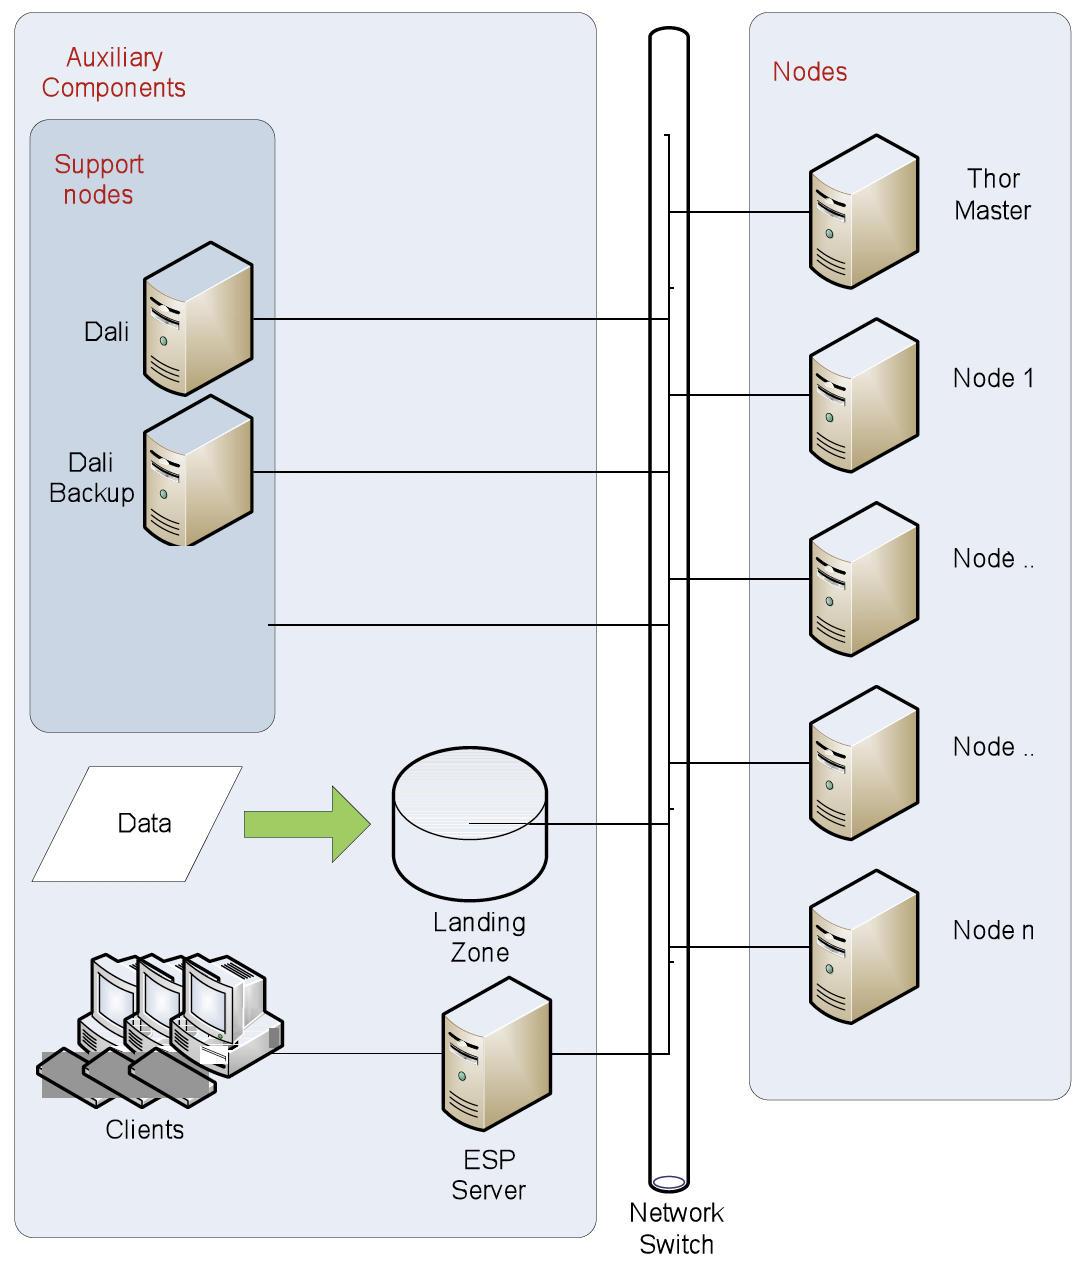
\includegraphics[width=\columnwidth]{images/thor.png}
\caption{The general Thor structure}\label{f:thor}
\end{figure}

Just like the Hadoop and other distributed computing, the Thor system also has the master/slave structure: in the Thor system, the single master node manages the parallel jobs in each slave nodes, each slave node executes a partial job of data refining. The outlier \textit{middleware} for data storing stores the processed data from the Thor system, and ECL server will manipulate query from developers directly on each slave nodes~\cite{Intro4}. The DFS (distributed file system) of the Thor gives flexible file format to the system; the data that stores could be stores in different formats. The computational power of the HPCC system could also be enhanced by the scale of the Thor system; a HPCC system cloud have flexible amount of the Thor systems. a HPCC system would be more efficient if there are more Thor systems~\cite{Intro4}.

\subsection{Roxie System - Data Delivery}
Roxie (Rapid Data Delivery Engine) system is designed for fast query in parallel computing cluster. One of the main reasons that the Roxie has great performance of searching and querying is because the pre-build indexed data system from the Thor system, another reason is the Roxie system uses the improved B+ tree to store data. The pre-processing step in the Thor system, and the data storage structure of the Roxie system are two important factors that generate high performance computing cluster~\cite{Intro4}.  

\begin{figure}[!ht]
\centering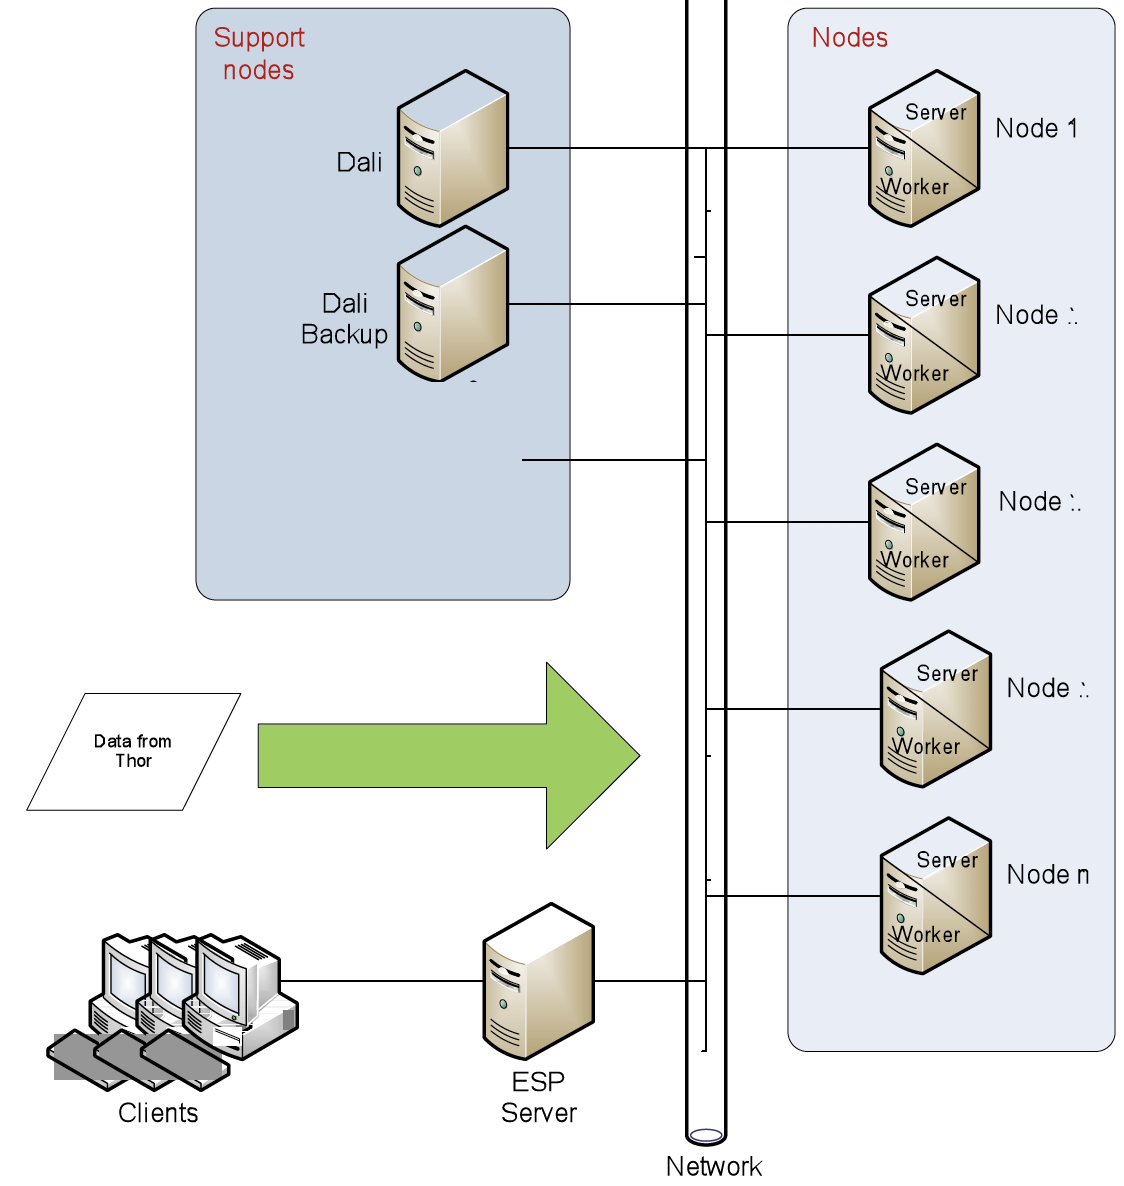
\includegraphics[width=\columnwidth]{images/roxie.png}
\caption{The general Roxie structure}\label{f:roxie}
\end{figure}

The Figure ~\ref{f:roxie} shows the basic structure of the Roxie system. The Roxie system follows the principle of Server and Agent processes: each server and agent construct a node, in the node, the server process takes querying requests through web protocols (distributed system), and at the same time, the Agent accepts the requests and processes the data queries. Same as the storage flexibility of the Thor, the Roxie system can also stores the data in different types, and in a HPCC system, the amount of Roxie is also configurable. However, in a HPCC system, the Roxie systems are rely on the Thor systems, since the Thor processing data for Roxie to manipulate. In other words: without the Thor, the Roxie is completely useless~\cite{Intro4}.

\subsection{The ECL Programming Language}

The Thor and Roxie systems are powerful systems and necessary component for the HPCC system platform, but without modified fo the procedures of the systems jobs, the whole HPCC system would not be functioning as expectation. Indeed, as the \textit{controller} of both Thor and Roxie systems, the ECL programming language is the main component which affects the performance and flexibility of the HPCC system. According to the official documentation of the ECL programming language:

``ECL is best described as a heavily optimized, data-centric declarative language. Exactly
what that means is detailed below; but the essence is that it is a language specifically designed to allow data
operations to be specified in a manner which is easy to optimize and parallelize.''~\cite{ECL}


The ECL is a declarative programming language, similar to SQL and XQuery, but the syntax of the ECL also reflects some intuition of other programming languages, such as Java, C++, and SQL~\cite{ECL}. As a declarative programming language, in order to run, it needs to be complied into another low-level language which could works on the hardware level. Despite the fact that the ECL is a declarative programming language, it has conquered many restrictions of programming language level, which makes the ECL easy to learn, and also has magnificent querying performance. Furthermore, the syntax design of the ECL itself also gives the ECL unique flavor, which lower the learning and developing cost potentially. ~\cite{ECL}

\section{Compare with Hadoop and MapReduce}

The HPCC system is a advanced high performance computing system which is perfectly for large scale of data processing and analyzing. Comparing with traditional parallelized computing platforms, such as Hadoop, MapReduce, There are three main advantages of the HPCC system for dealing with large data scale~\cite{Intro4}:

\begin{itemize}
	\item Flexibility: The HPCC is a flexible system, which could has self-defined architecture of processing data, but the traditional computing platform such as MapReduce has strict architecture, which is less likely to adopt customized methods.
	\item System Integrity: The HPCC is a unique system, which could executing by itself, unlike Hadoop and MapReduce, which need to run on another system base.
	\item Fast Online Querying Ability: Since the HPCC is designed as a network-based distributed computing system, with the power of the core (Thor, Roxie, ECL), it has more advantage in fast querying online, and the HPCC could also supports more users at the same time with efficient querying ability.
\end{itemize}

\section{Conclusion}

The HPCC is a efficient, open source, and developer-friendly systems, it has great performance on processing large scale of data, which is a perfect tool for the amount of data and information need to be processed in nowaday. The key components of the HPCC system are Thor systems, Roxie systems, and ECL programming languages. The three components works together, and bring the HPCC system remarkable performance. Compare with Hadoop and MapReduce, the HPCC is more suitable for commercial usage, because of the flexibility, system integrity, and rapid querying ability.

Although, this paper does not include the data integrity of the HPCC system. Since the HPCC is a distributed data processing system, the data integrity is an important topic that need to be discuss, especially to protect the business secret of the commercial usage.

\begin{acks}

  The authors would like to thank Dr.~Gregor~von~Laszewski for his
  support and suggestions to write this paper.

\end{acks}

\bibliographystyle{ACM-Reference-Format}
\bibliography{report} 

